\section{实验}
\label{sec:experiments}

所有加速比均定义为基线时间除以 DrainSinkhorn 时间。OT 阶段时间直接测量，或通过从包含 OT 的已记录区间中减去配对消费者时间来重构。对于重构结果，先在每个配对计时单元内部减去消费者时间，再计算比率、区间或 bootstrap 汇总。匹配组件比较固定输入、proposal、容差、验证检查时点、双边际验证器和消费者。完整路径比较在两臂中使用相同的 packed 或 vectorized 后端。当停止控制器产生不同的实际残差时，论文同时报告实际残差和消费者输出偏差。

因此，本文报告的比率具有两个因果作用：
\[
\begin{gathered}
\underbrace{\text{固定宽度}\rightarrow\text{动态压缩}}_{\text{释放与动态压缩}},\\[-1pt]
\underbrace{\text{逻辑 mask}\rightarrow\text{动态压缩}}_{\text{宽度效应}}.
\end{gathered}
\]
固定宽度/动态压缩测量从普通固定宽度批次到动态压缩控制器的净变化；logical-mask/dynamic-compaction（LM/DC）则在匹配释放决策下隔离动态缩宽。\Cref{fig:main-results-width} 报告实测宽度成本曲线，表~\ref{tab:main-results-by-width} 按初始宽度组织已登记效应。附录表~\ref{tab:attribution-map} 列出每个对照的实现、计时范围和统计单元。冻结 workload 上的 bootstrap 区间量化给定冻结输入和执行配置下的计时可复现性。每个对照均在所列实验及测量区间内解释。

\begin{figure*}[!t]
\centering
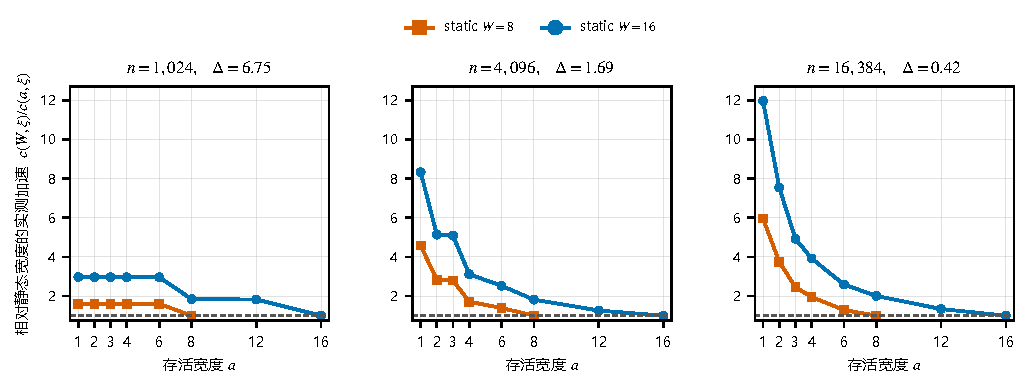
\includegraphics[width=\textwidth]{figures/MAIN_RESULTS_WIDTH_COST_ZH.pdf}
\caption{从存活宽度到 packed-update 加速的实测转化。每条曲线报告相对静态宽度 $W\in\{8,16\}$ 的 $g_W(a)=c(W,\xi)/c(a,\xi)$；所有面板使用相同坐标轴，阴影由 30 次重复的逐宽度四分位端点传播得到。面板标题给出决定 scheduling-wave 量化的 $\Delta=b_mN_{\mathrm{SM}}/n$。}
\label{fig:main-results-width}
\end{figure*}
\begin{table*}[!t]
\centering
\caption{按初始宽度分组的已登记匹配结果。加速比定义为基线时间除以动态压缩时间。方括号为已登记 95\% 区间，圆括号为观测 seed 或 plan 范围。各行保留所属 campaign 的计时范围，不跨行合并。逐行来源记录在 \texttt{support/figure\_materials/MAIN\_RESULTS\_BY\_WIDTH.csv}。}
\label{tab:main-results-by-width}
\scriptsize
\setlength{\tabcolsep}{3.3pt}
\begin{tabular}{@{}cllllp{4.0cm}@{}}
\toprule
$W$ & Campaign & Workload ($n$) & 对照 & 加速比 & 计时范围与统计单元 \\
\midrule
% Source: manuscript/forgetting_ot_e2e_closure/support/figure_materials/C63_SOLVER_ATTRIBUTION.csv
8 & C63 & ImageNet-32 ($1024$) & fixed/DC & $1.054\times$ (1.033--1.072) & solver field；3 个训练 seed \\
% Source: studies/campaigns/C62_semantic_latent_OTFM_four_arm/manifest.json
8 & C62 & ImageNet-32 ($1024$) & fixed/DC & $1.105\times$ (1.079--1.156) & coupling 准备；3 个 problem--plan seed \\
% Source: knowledge/audits/DRAINSINKHORN_ACCURACY_CONTRACT_AND_SPEEDUP_AUDIT_20260828_ZH.md
8 & C80-LM & Packer19 ($16384$) & LM/DC & $1.5397\times$ [1.5389, 1.5404] & 扣除 consumer 的 OT 阶段；24 个配对单元 \\
% Source: manuscript/forgetting_ot_e2e_closure/support/figure_materials/PACKER19_STOPPING_METRICS.csv
8 & EXP-P19 & Packer19 ($16384$) & LM/DC & $1.5713\times$ [1.5701, 1.5726] & 直接 OT 阶段；24 个配对单元 \\
% Source: knowledge/audits/C67_GLOBAL8_TWO_HOST_RESULT_20260828_ZH.md
8 & C67-F3 & MetroPT-3 ($16384$) & fixed/DC & $2.159\times$ & 八 worker 完整端点；每 worker 固定 workload \\
% Source: knowledge/audits/C67_GLOBAL8_TWO_HOST_RESULT_20260828_ZH.md
8 & C67-F2 & MetroPT-3 ($16384$) & fixed/DC & $3.110\times$ & 八 worker 完整端点；每 worker 固定 workload \\
\midrule
% Source: studies/campaigns/C33_ImageNet32_independent_8GPU_Flash_policy_gate/manifest.json
16 & C33 & ImageNet-32 ($4096$) & fixed/DC & $1.421\times$ & 稳态关键路径；40 个窗口 \\
% Source: studies/campaigns/C55_OTTJAX_ImageNet32_relaxed_phase_active/manifest.json
16 & C55 & ImageNet-32 ($4096$) & fixed/DC & $1.581\times$ & 匹配的 20-update phase；10 次重复 \\
% Source: studies/campaigns/C67_MetroPT3_fully_matched_scaling/manifest.json
16 & C67-32k & MetroPT-3 ($32768$) & fixed/DC & $1.616\times$ & 单 worker 端点；equal-host 几何均值 \\
% Source: studies/campaigns/C66_release_fair_Flash_generation_matrix/manifest.json
16 & C66 & MetroPT-3 ($16384$) & fixed/DC & $1.7447\times$ [1.7434, 1.7467] & 双主机 ready-arrays-to-consumer 端点 \\
% Source: studies/campaigns/C82_MetroPT3_static_active_corrected/analysis.json
16 & C82 & MetroPT-3 ($16384$) & fixed/DC & $1.7455\times$ (1.7453--1.7460) & 四 worker makespan；3 个已登记 plan \\
% Source: studies/campaigns/C67_MetroPT3_fully_matched_scaling/manifest.json
16 & C67-8k & MetroPT-3 ($8192$) & fixed/DC & $2.316\times$ & 单 worker 端点；equal-host 几何均值 \\
\bottomrule
\end{tabular}
\end{table*}

\subsection{匹配的释放与动态压缩}

匹配比较从常规固定宽度批量执行开始。C82 在一台主机的四个完整设备 worker 上直接比较两条当前 MetroPT-3 路径。动态压缩在 ready-arrays-to-consumer 端点上达到 \CMetroCorrectedEndpointSpeedup{}，同时问题更新槽位从 \CMetroSlotsStatic{} 降至 \CMetroSlotsActive{}。三个预声明执行 plan 均支持动态压缩路径，描述性范围为 \CMetroCorrectedEndpointRange{}。两臂在每个 repeat 中都调用 16 个 verifier candidate、验证 16 个 candidate，并启动 32 个 plan-application kernel。相应的四 GPU 能耗比为 \CMetroCorrectedEnergyFactor{}。

C66 提供独立的双主机匹配研究。其固定宽度/动态压缩比在 E2 端点上为 $1.744723\times$；在每个 host--plan 单元内扣除配对 consumer 后，E1 比率为 \CMetroRetirementOTSpeedup{}。六个 host--plan 单元均支持动态压缩路径。

C67 把相同的完整设备设计扩展到两台主机上的八个独立 worker。两个 fixed-per-worker 端点单元的匹配固定宽度/动态压缩加速分别为 $3.110\times$ 与 $2.159\times$，同时按 \cref{tab:c67-global8} 降低 slots。另有两个在两台主机均通过冻结门的单 worker support-size 单元：$n=8192$ 时为 $2.316\times$，$n=32768$ 时为 $1.616\times$。

\begin{table}[t]
\centering
\caption{C67 在两台主机的八个完整设备 worker 上执行 fixed-per-worker 实验。时间汇总完整 consumer 端点。Slots 统计跨 worker 的问题更新；能耗使用同一端点。}
\label{tab:c67-global8}
\scriptsize
\setlength{\tabcolsep}{3pt}
\resizebox{\columnwidth}{!}{%
\begin{tabular}{@{}lrrrrr@{}}
\toprule
路线 & 固定宽度 (s) & 动态压缩(s) & Slots 固定/动态 & 时间比 & 能耗比 \\
\midrule
failure-2 & 12.523 & 4.026 & 4736 / 1276 & 3.110$\times$ & 3.437$\times$ \\
failure-3 & 7.999 & 3.705 & 3008 / 1244 & 2.159$\times$ & 2.292$\times$ \\
\bottomrule
\end{tabular}}
\end{table}


在 C63 中，每个训练 step 使用真实 ImageNet-32 PCA500 特征 coupling。\cref{tab:absolute-ot-times} 报告四条路径的 solver 阶段时间。配对 solver-field 固定宽度/动态压缩为 $1.054\times$（观测 seed 范围 $1.033$--$1.072\times$；\cref{tab:c63-solver-pairs}）。在完整 fixed-update 训练区间上，固定宽度/动态压缩为 \CFeatureTrainingActiveOverStatic{}（范围 \CFeatureTrainingActiveOverStaticRange{}）。C62 单独测量三个 problem-plan seed 上的 coupling 准备，固定宽度/动态压缩为 $1.105\times$。使用一个初始化处理多个问题的实验给出非冷启动条件：在 40 个受控重叠 support 窗口上，动态压缩路径加速 $1.421\times$、slots 减少 30.62\%，并在全部配对窗口中获胜。

\begin{table*}[t]
\centering
\caption{经过 50k 次训练更新后的 ImageNet-32 PCA500 特征空间质量。表中给出匹配固定宽度（Fixed）与动态压缩（Dynamic）执行的三个 seed 均值；三项指标均为越低越好。质量评估始终使用相同的三个配对训练 seed；完整逐 seed 测量值与分析文件已放在公开 GitHub 仓库中。这些是特征空间指标，不是像素空间 FID。}
\label{tab:imagenet-quality}
\small
\begin{tabular}{@{}c cc cc cc@{}}
\toprule
& \multicolumn{2}{c}{曲率} & \multicolumn{2}{c}{Held-out FM MSE} & \multicolumn{2}{c}{Projected Fr\'echet} \\
NFE & Fixed & Dynamic & Fixed & Dynamic & Fixed & Dynamic \\
\midrule
4  & 5.4524 & 5.4448 & 1.07854 & 1.07859 & 1.2967 & 1.2886 \\
8  & 2.8388 & 2.8356 & 1.07854 & 1.07859 & 1.5286 & 1.5224 \\
16 & 1.4546 & 1.4528 & 1.07854 & 1.07859 & 1.8182 & 1.8136 \\
\bottomrule
\end{tabular}
\end{table*}


这些数值质量结果在 NFE 4、8 与 16 下始终使用相同的三个配对训练 seed。完整逐 seed 测量值与分析文件已放在公开 GitHub 仓库（\url{https://github.com/cis-aconiticacid/DrainSinkhorn}）中。该评估测量 ImageNet-32 PCA500 特征空间 OT-FM 端点。

\subsection{从宽度到 kernel 时间的实测转化}

我们通过在固定问题规模下调用同一个 packed Triton 更新、只改变宽度，测量式 \eqref{eq:time-difference} 中的宽度成本项。\Cref{fig:main-results-width} 将实测中位数归一化为静态宽度 $W=8$ 与 $16$ 下的 $g_W(a)=c(W,\xi)/c(a,\xi)$，并统一使用存活宽度坐标 $a\in\{1,2,3,4,6,8,12,16\}$。对实际存活宽度 $A_k$，式 \eqref{eq:time-difference} 中对应的单项为 $c(W,\xi_k)[1-g_W(A_k)^{-1}]$。面板值 $\Delta=b_mN_{\mathrm{SM}}/n$ 预测平台尺度：$n=1024$ 时转化受到明显量化（$\Delta=6.75$），$n=4096$ 时量化变细（$\Delta=1.69$），$n=16384$ 时接近连续转化（$\Delta=0.42$）。

该诊断隔离 packed update，因此估计的是 $c_k(a,\xi_k)$ 的一个组成部分，而不是完整执行器。它在 $n=1024,W=8$ 下的形状与较小的 C63 solver-field 比率一致：存活宽度进入 $A\leq6$ 区域后，继续移除 lane 对槽位数的影响大于对 packed-update 时间的影响。$n=16384$ 的响应则提供较大 MetroPT-3 动态压缩收益所需的硬件条件；匹配的 C82 端点进一步测量包含控制与消费者工作的完整净效应。

\paragraph{跨后端家族迁移。}
OTT-JAX 与 PyKeOps 结果通过独立实现测试执行原理。在真实 ImageNet-32、$W=16$ 上，每个固定阶段只处理剩余问题的 OTT-JAX 执行比原生 OTT-JAX 快 \COTTNativeActiveSpeedup{}；匹配的固定宽度/动态压缩对照将其中 \COTTStaticActiveSpeedup{} 归因于只在阶段边界移除已完成问题并重新划分存活问题。在真实 A2D2 LiDAR、$W=8$ 上，PyKeOps active 路径比 sequential carry 快 \CKeopsLiDARActiveSpeedup{}。真实 ImageNet-32 PyKeOps 单元仍取得 \CKeopsImageNetActiveSpeedup{} 正收益。tiled-log 实现在不实例化候选 kernel 的情况下扩展到 $n=65536$，给出实测容量边界。

独立 OTT-JAX 与 PyKeOps 实现汇总于 \cref{tab:ot-cross-backend}。

\subsection{Packer19 停止与执行 Pareto}

双主机 EXP-PACKER19 实验评估 $10^{-4}$、$3\times10^{-4}$、$10^{-3}$、$3\times10^{-3}$ 和 $10^{-2}$ 残差容差，并且不跨容差聚合。所有实验臂使用相同的双边际验证器与残差容差，以及相同的紧参考消费者输出。

\begin{figure*}[t]
\centering
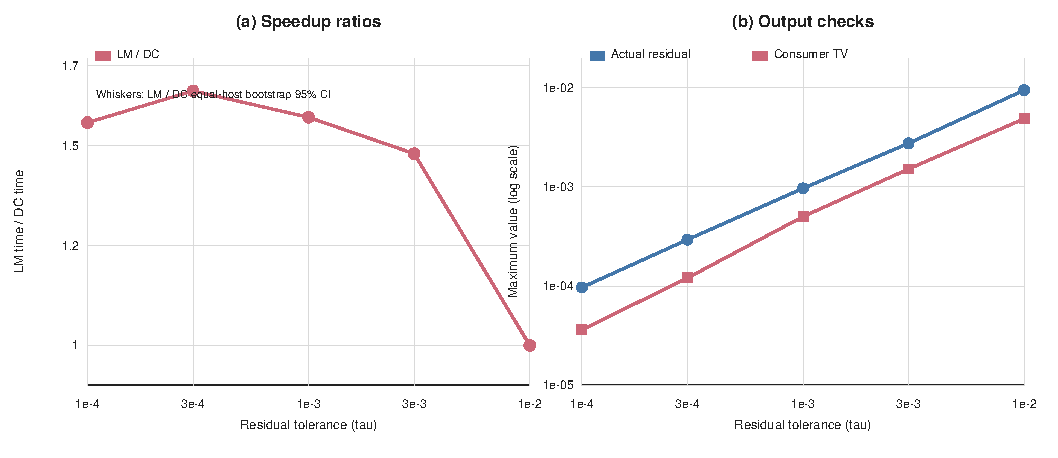
\includegraphics[width=\textwidth]{../forgetting_ot_e2e_closure/figures/PACKER19_STOPPING_METRICS.pdf}
\caption{使用相同双边际验证器与残差容差的双主机 Packer19 停止--执行结果。面板 (a) 展示五个容差下的 LM/DC 速度比，误差线为 equal-host 分层 bootstrap 95\% 区间。面板 (b) 以对数纵轴展示最大实际残差和最大 consumer TV。每个点汇总 24 个配对单元；consumer TV 检查相对紧参考的输出差异。}
\label{fig:packer-stopping-metrics}
\end{figure*}

在 $10^{-4}$ 至 $3\times10^{-3}$，动态压缩相对逻辑 masking 提升 \CPackerCompactionRange{}。在 $10^{-2}$，全部八个问题都在第 8 次更新首次通过，因此不存在可移除的 padding，LM/DC 为中性的 \CPackerNeutralCompaction{}（95\% CI \CPackerNeutralCompactionCI{}）。这些有效对照刻画 EXP-PACKER19 的动态压缩路径与逻辑 mask 路径；较早 C80-LM 的对照与阶段成本分别见 \cref{tab:c80-attribution,tab:phase-costs}。

所有已登记端点质量检查均通过。

\subsection{匹配组件归因}

\paragraph{释放与动态压缩的效应。}
C82 在匹配 MetroPT-3 E2 端点上得到 \CMetroCorrectedEndpointSpeedup{}；C66 在单独测量的 E1 OT 阶段上得到 \CMetroRetirementOTSpeedup{}。在 C63 ImageNet-32 四臂训练消融中，动态压缩在三个 seed 上相对固定宽度 batching 增加 \CFeatureTrainingActiveOverStatic{}（区间 \CFeatureTrainingActiveOverStaticRange{}）。这是 E3 端点归因；$1.054\times$ 的 C63 solver-field 对照单独报告在 \cref{tab:absolute-ot-times,tab:c63-solver-pairs}。

C80 与 C80-LM 在两台主机上使用相同的 Packer19 单细胞转移 workload，每台主机包含四张 A100-SXM4-80GB。三种冻结方法顺序产生 24 个配对的 host--order--GPU 单元。每个单元使用排除 warmup 后的重复中位数、相同输入、packed-kernel source tree、$10^{-3}$ 停止容差和转移消费者。

\begin{table}[t]
\centering
\caption{在一个冻结输入和 release contract 下，Packer19 的单变量归因。每行都报告扣除配对消费者后的 OT 阶段时间，因此各组件效应使用同一测量边界。}
\label{tab:c80-attribution}
\scriptsize
\setlength{\tabcolsep}{2.6pt}
\resizebox{\columnwidth}{!}{%
\begin{tabular}{@{}lllll@{}}
\toprule
改变 & 匹配对照 & 范围 & 比率 & 证据 \\
\midrule
批量验证检查 & serial / batched verifier & OT 阶段 & 1.133$\times$ & 24/24 胜出 \\
当前边缘初步检查 & 仅验证器 / 先初步检查 & OT 阶段 & 1.105$\times$ & 24/24 胜出 \\
逻辑冻结 & fixed / logical mask & OT 阶段 & 1.000$\times$ & 95\% CI [0.9998, 1.0003] \\
动态压缩& logical mask / dynamic compaction & OT 阶段 & \CPackerCompactionOTSpeedup{} & 95\% CI \CPackerCompactionOTRange{} \\
\bottomrule
\end{tabular}}
\vspace{2pt}

{\scriptsize 批量验证检查与当前边缘初步检查两行均为 24/24 配对胜出；这两个对照没有登记独立的 E1 bootstrap 区间。}
\end{table}


\paragraph{检查与 screening。}
对照暴露出不同工作。批量执行双边际验证器以及使用当前边缘进行初步检查，在匹配路径下降低 OT 阶段时间。每个 C80 比率都先减去其配对消费者时间，再形成比较。

我们重放全部 \CPackerShadowNegatives{} 个预检为负的事件，并逐一使用双边际验证器检查，发现其中 \CPackerShadowMissedReady{} 条 lane 已经可以释放。初步检查与验证器的行残差最大差异为 \CPackerScreenDiscrepancy{}。每个输出 plan 都以 $10^{-3}$ 通过双边际验证器。

\paragraph{逻辑 masking 与动态压缩。}
在 C80-LM 中，逻辑 masking 为中性，因为 packed kernel 仍保持宽度 8。动态压缩降低观测宽度，移除 256 个问题更新槽位中的 100 个，并产生 \CPackerCompactionOTSpeedup{} OT 阶段加速，区间为 \CPackerCompactionOTRange{}。全部 24 个配对单元均支持动态压缩。在 24 个 host--order--GPU 单元中位数上，端点能耗从 879.9 J 降至 688.1 J，而压缩后的 buffer 会把峰值 allocated memory 从 80.8 MiB 提高到 106.9 MiB。

\subsection{运行区间：异质性与宽度}

M3 固定 32 个真实 MetroPT 问题的集合，只改变它们进入窗口的分组。离线逐循环迭代编号 $q_t$ 定义分组，验证器给出的迭代编号 $n_t$ 测量实际执行工作。Oracle homogeneous grouping 最小化每个窗口内所需迭代编号的差异。Heterogeneous 与 random grouping 增大静态矩形和由 $n_t$ 定义的生存曲线之间的面积。匹配的固定宽度/动态压缩比率从 \CMThreeHomogeneousRetirementSpeedup{} 上升到 \CMThreeHeterogeneousRetirementSpeedup{}，random layout 上为 $1.235$--$1.271\times$。

\begin{table}[t]
\centering
\caption{对同一固定真实任务 multiset 的 M3 分组干预。对于窗口内的离线逐循环迭代编号 $q_s$，$H_q=\operatorname{sd}(q_s)/\operatorname{mean}(q_s)$，padding 为 $W\max_s q_s/\sum_s q_s-1$。Dynamic slot 是动态压缩相对固定宽度的候选迭代槽位比。表中数值对窗口汇总；timing repeat 用于稳定每种条件，并非独立数据集。}
\label{tab:m3-grouping}
\scriptsize
\setlength{\tabcolsep}{3pt}
\begin{tabular}{@{}lcccc@{}}
\toprule
分组 & $H_q$ & Padding & Dynamic slot & 固定/动态 \\
\midrule
heterogeneous & 0.236 & 0.236 & 0.802 & 1.217$\times$ \\
homogeneous & 0.127 & 0.110 & 0.892 & 1.105$\times$ \\
random 1 & 0.254 & 0.293 & 0.776 & 1.258$\times$ \\
random 2 & 0.264 & 0.270 & 0.789 & 1.235$\times$ \\
random 3 & 0.260 & 0.279 & 0.764 & 1.271$\times$ \\
\bottomrule
\end{tabular}
\end{table}


\paragraph{独立有限精度压力测试。}
C10 在 1/2/4/8 GPU 上测量 84 个阈值附近候选和 16 个运行时攻击的决策行为。相对独立 FP64 replay，raw FP32 与 TF32 各有三个 accept decision 不一致；outward-bound guard 随后执行 FP64 escalation，在这 100 个 case 中没有不一致。该 guarded 配置与正式计时的应用分开评估。

\paragraph{正式计时的应用与独立 worker scale-out。}
正式计时的 packed Triton 路径使用后端支持的精度和双边际验证器。所有输出 plan 均满足记录的行、列边缘残差界限，且每个端点均通过登记的输出或质量门。C67 把完整窗口分配给独立 GPU worker。四个 worker 在 held-out MetroPT route 上取得 $3.965$--$3.979\times$ fixed-per-worker throughput scaling，worker 之间没有 Sinkhorn collective；八 worker 的匹配端点分解见 \cref{tab:c67-global8}。
